\begin{figure}[tbp]
\centering
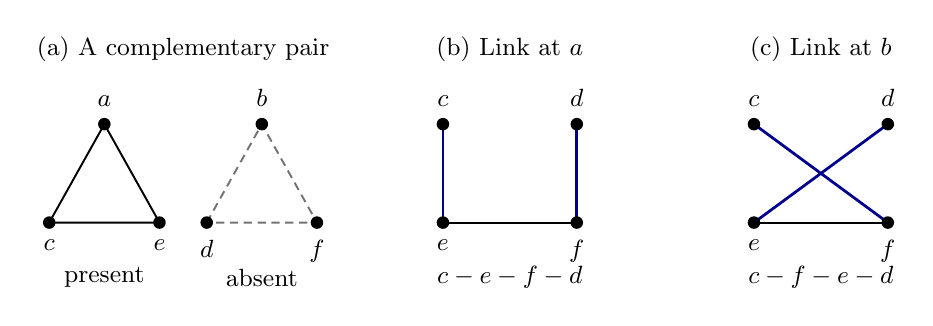
\begin{tikzpicture}[
  x=1cm,y=1cm,font=\small,
  vertex/.style={circle,fill=black,inner sep=1.6pt},
  every path/.style={line width=.7pt},
  matching/.style={draw=blue!55!black,line width=1pt}
]
\node at (1.7,2.2) {(a) A complementary pair};
\node at (5.85,2.2) {(b) Link at $a$};
\node at (9.8,2.2) {(c) Link at $b$};
\draw (0,0)--(.7,1.25)--(1.4,0)--cycle;
\node[vertex,label=above:$a$] at (.7,1.25) {};
\node[vertex,label=below:$c$] at (0,0) {};
\node[vertex,label=below:$e$] at (1.4,0) {};
\draw[densely dashed,draw=black!55] (2,0)--(2.7,1.25)--(3.4,0)--cycle;
\node[vertex,label=above:$b$] at (2.7,1.25) {};
\node[vertex,label=below:$d$] at (2,0) {};
\node[vertex,label=below:$f$] at (3.4,0) {};
\node at (.7,-.7) {present};
\node at (2.7,-.7) {absent};
\draw (5,0)--(6.7,0);
\draw[matching] (5,1.25)--(5,0) (6.7,0)--(6.7,1.25);
\node[vertex,label=above:$c$] at (5,1.25) {};
\node[vertex,label=above:$d$] at (6.7,1.25) {};
\node[vertex,label=below:$e$] at (5,0) {};
\node[vertex,label=below:$f$] at (6.7,0) {};
\node at (5.85,-.7) {$c-e-f-d$};
\draw (8.95,0)--(10.65,0);
\draw[matching] (8.95,1.25)--(10.65,0) (8.95,0)--(10.65,1.25);
\node[vertex,label=above:$c$] at (8.95,1.25) {};
\node[vertex,label=above:$d$] at (10.65,1.25) {};
\node[vertex,label=below:$e$] at (8.95,0) {};
\node[vertex,label=below:$f$] at (10.65,0) {};
\node at (9.8,-.7) {$c-f-e-d$};
\end{tikzpicture}
\caption{The complementary-triple rule forces opposite matchings.
Suppose the two triangles through $\{a,b\}$ are $\{a,b,c\}$ and
$\{a,b,d\}$. The links at $a$ and $b$, restricted to
$\{c,d,e,f\}$, share the edge $\{e,f\}$ and use opposite matchings
between $\{c,d\}$ and $\{e,f\}$ (shown in blue).
One of the two possible choices is drawn. The crossing in (c) is not a
vertex. Panel (a) shows one complementary pair for this choice.}
\label{fig:six-label-paths}
\end{figure}
